\section{Experimental Results}
\ifCLASSOPTIONonecolumn\begin{figure*}[t]
\centering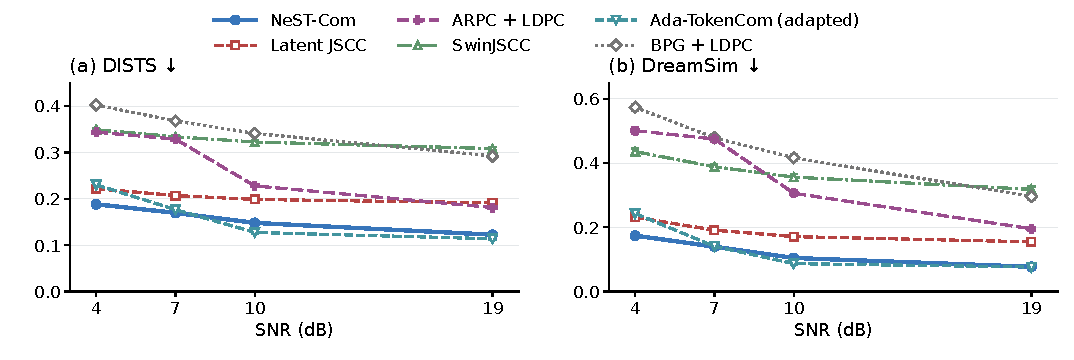
\includegraphics[width=\textwidth]{figure2.pdf}
\caption{Six-system reconstruction on common500 at $N=1024$. Points and bars are equal-source means and pointwise 95\% source-bootstrap intervals after averaging three channel realizations per source, including failures. Ada is the predicted-class, fixed-frame adaptation. Lower DISTS and DreamSim are favorable.}
\label{fig:performance}
\end{figure*}
\fi
\subsection{Experimental Setup}
The 500 ImageNet validation sources~\cite{imagenet} are disjoint from cal1000 and use fixed $256\times256$ preprocessing. We evaluate $N=1024$ at 4/7/10/19 dB and $N=512$ at 4/10/19 dB. Each point averages three channel realizations per source, retaining gray failures, before equal-source means and direct paired 95\% source-bootstrap intervals (10\,000 resamples). Controls use the first 100 full manifest IDs. Historical noise identities remain method/budget-specific; the matched-grid control shares noise.

Latent JSCC maps tokenizer latents to symbols with convolutional layers and shares $\Dc$, using MSE, LPIPS, and latent-consistency losses (100k updates). SwinJSCC~\cite{swinjscc} uses RGB MSE (200k updates, minimum calibration MSE selection). Both train on 20\,000 images for $256\times256$ and $N=1024$. Digital baselines include BPG~\cite{bpg} and ARPC~\cite{arpc} with LDPC/QAM. The predicted-class, fixed-frame Ada-TokenCom adaptation~\cite{adatokencom} retains LlamaGen-L/VQ16, prefix arithmetic coding, and sampled completion (CFG=4, $T=1$, top-$k=2000$, top-$p=1$). ConvNeXt predicts its transmitted 10-bit class; ARPC captions and all required fields are likewise paid. This comparison does not reproduce Ada's long-term budget controller or ARQ.

DISTS~\cite{dists} and DreamSim~\cite{dreamsim} measure source-referenced structure/texture and perceptual distance. We also report PSNR, LPIPS-Alex~\cite{lpips}, and CLIP-I~\cite{clip}. Metrics use native floating-point RGB: DISTS uses $256\times256$ without resizing; DreamSim/CLIP use the frozen $224\times224$ bicubic-antialias preprocessing. DINO-based calibration and feature-based evaluation are related criteria, rather than independent perceptual judgments. All models and numeric routes are frozen; Supplement~S1 specifies policies and the differing calibration pools.

\ifCLASSOPTIONonecolumn\else\begin{figure*}[t]
\centering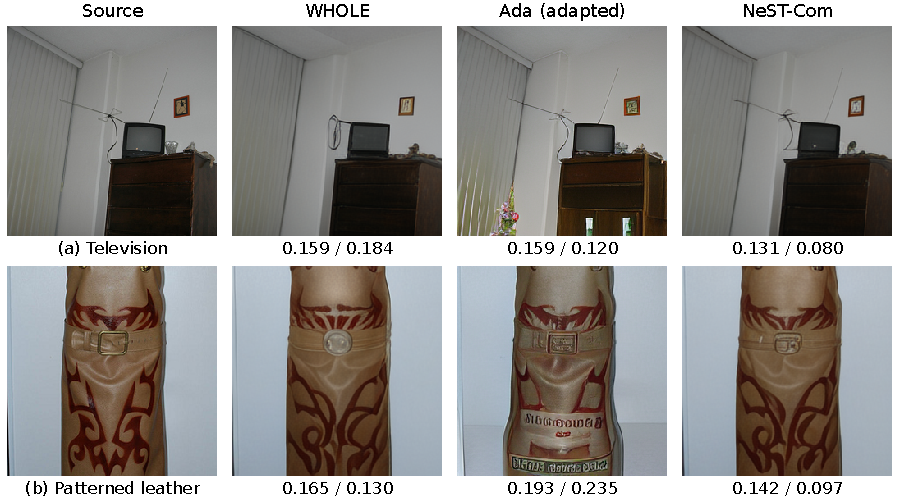
\includegraphics[width=6.0in]{figure3.pdf}
\caption{Selected qualitative examples at $N=1024$ and 7 dB. Columns show source, WHOLE, fixed-frame Ada, and NeST-Com. These examples illustrate visible advantages rather than a random sample. Each uses the fixed first channel realization for that method. Values are DISTS$\downarrow$ / DreamSim$\downarrow$ for the displayed full-field output.}
\label{fig:qualitative}
\end{figure*}
\fi
\subsection{Effect of Within-Scale Transmission}
\begin{table}[t]
\caption{Within-scale transmission evidence. (A) NeST minus WHOLE under the frozen family policies. (B) Only endpoint granularity changes under matched model, MCS, ceiling, and noise. (C) Ordered receiver interventions on the actual NeST prefixes. Brackets are source-paired 95\% intervals; each block uses its stated population.}
\label{tab:internal}\centering\footnotesize
\setlength{\tabcolsep}{2.1pt}\renewcommand{\arraystretch}{1.05}
\begin{tabular}{@{}lccc@{}}\toprule
\multicolumn{4}{l}{\textit{A. common500, $N=1024$, family-specific policies}}\\
SNR & Util. W$\to$N (\%) & $\Delta$DISTS & $\Delta$DreamSim\\
\midrule
4 & 73.81$\to$99.56 & \shortstack{-0.0146\\{}[-0.0157, -0.0136]} & \shortstack{-0.0303\\{}[-0.0333, -0.0273]}\\[2pt]
7 & 83.19$\to$99.75 & \shortstack{-0.0060\\{}[-0.0097, -0.0021]} & \shortstack{-0.0108\\{}[-0.0157, -0.0057]}\\[2pt]
10 & 77.70$\to$99.79 & \shortstack{-0.0141\\{}[-0.0153, -0.0128]} & \shortstack{-0.0270\\{}[-0.0299, -0.0241]}\\[2pt]
19 & 85.24$\to$99.83 & \shortstack{-0.0048\\{}[-0.0053, -0.0043]} & \shortstack{-0.0043\\{}[-0.0051, -0.0036]}\\[2pt]
\midrule
\multicolumn{4}{l}{\textit{B. control100, 10 dB, common ceiling $(8,126)$}}\\
Grid (ends) & Utilization (\%) & DISTS & DreamSim\\
\midrule
Whole (5) & 78.13 & 0.1650 & 0.1387\\
Quarter (20) & 95.19 & 0.1535 & 0.1143\\
Eighth (39) & 97.44 & 0.1516 & 0.1137\\
Token (352) & 99.85 & 0.1505 & 0.1115\\
\midrule
\multicolumn{4}{l}{\textit{C. control100, 10 dB, same received prefixes}}\\
Intervention & $\Delta$PSNR (dB) & $\Delta$DISTS & $\Delta$DreamSim\\
\midrule
B0--A0 & \shortstack{+0.287\\{}[0.240, 0.335]} & \shortstack{-0.0062\\{}[-0.0077, -0.0048]} & \shortstack{-0.0113\\{}[-0.0147, -0.0083]}\\[2pt]
C0--B0 & \shortstack{+0.537\\{}[0.404, 0.682]} & \shortstack{-0.0083\\{}[-0.0102, -0.0065]} & \shortstack{-0.0159\\{}[-0.0205, -0.0116]}\\[2pt]
\bottomrule\end{tabular}\end{table}

Table~\ref{tab:internal}(A) compares the shared tokenizer, prior, coder, and receiver under frozen family policies. At $N=1024$, 10 dB, token-wise transmission increases utilization from 77.70\% to 99.79\%. Its paired DISTS and DreamSim differences are $-0.0141\,[-0.0153,-0.0128]$ and $-0.0270\,[-0.0299,-0.0241]$. All seven budget/SNR points favor NeST on both distances; PSNR gains over WHOLE range from 0.45 to 0.88 dB at $N=1024$.

Block B isolates endpoint granularity on 100 sources with fixed 16-QAM rate 2/3, maximum position $(8,126)$, and common noise. Quarter-to-Token refinement raises utilization from 95.19\% to 99.85\%, improving DISTS by $-0.0030\,[-0.0041,-0.0020]$, DreamSim by $-0.0028\,[-0.0050,-0.0006]$, and PSNR by $0.172\,[0.125,0.221]$ dB. The mean descending length comparisons are 1.55/4.51/7.57/125.96 for Whole/Quarter/Eighth/Token. These count cached-length comparisons, not neural forwards or elapsed time. Relative to the historical Quarter policies on common500, Token improves DISTS and DreamSim at six of seven points; the 7-dB intervals cross zero (Supplement~S2).

Block C holds the actual NeST prefixes fixed. A0 ignores the boundary correction but retains prior completion; B0 adds its residual correction while retaining the A0 conditioning path; C0 updates both. At 10 dB, B0--A0 and C0--B0 reduce DreamSim by $0.0113$ and $0.0159$, respectively, with intervals excluding zero. These ordered whole-boundary interventions do not partition the extra Token--Quarter gain. The 7-dB results and final-scale check are in Supplement~S3.

\subsection{Comparison With Existing Methods}
\ifCLASSOPTIONonecolumn\begin{figure*}[t]
\centering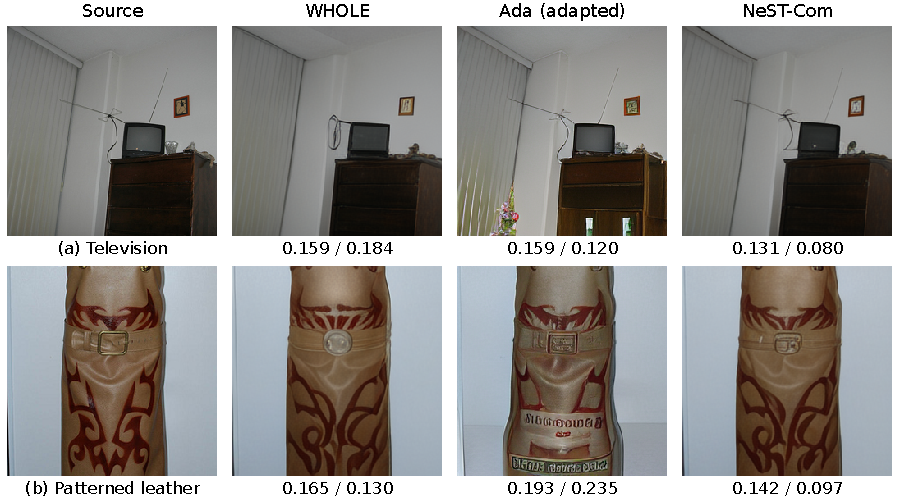
\includegraphics[width=6.0in]{figure3.pdf}
\caption{Selected qualitative examples at $N=1024$ and 7 dB. Columns show source, WHOLE, fixed-frame Ada, and NeST-Com. These examples illustrate visible advantages rather than a random sample. Each uses the fixed first channel realization for that method. Values are DISTS$\downarrow$ / DreamSim$\downarrow$ for the displayed full-field output.}
\label{fig:qualitative}
\end{figure*}
\fi
\begin{table}[t]
\caption{Auxiliary quality and processing costs at $N=1024$, 10 dB. Quality uses common500; timing uses 32 sources, one RTX PRO 6000, two CPU cores, batch one, and complete TX/RX processing boundaries. BPG uses CPU only.}
\label{tab:external}\centering\footnotesize\setlength{\tabcolsep}{2.5pt}
\begin{tabular}{@{}lrrrrr@{}}\toprule
Method & PSNR & LPIPS & CLIP-I & TX & RX\\
 & (dB)$\uparrow$ & $\downarrow$ & $\uparrow$ & (ms) & (ms)\\
\midrule
WHOLE & 19.31 & 0.199 & 0.858 & 213.8 & 369.9\\
NeST-Com & 20.19 & 0.166 & 0.877 & 248.4 & 411.6\\
Ada (adapted) & 19.56 & 0.167 & 0.884 & 7795.6 & 7626.1\\
Latent JSCC & 20.80 & 0.173 & 0.789 & 15.4 & 24.1\\
SwinJSCC & 23.03 & 0.469 & 0.669 & 20.5 & 17.6\\
BPG + LDPC & 22.54 & 0.589 & 0.635 & 2442.0 & 31.7\\
ARPC + LDPC & 16.47 & 0.341 & 0.713 & 661.7 & 797.0\\
\bottomrule\end{tabular}\end{table}

Fig.~\ref{fig:performance} compares six complete systems, whose tokenizer, prior, decoder, and conditioning differ. At 4 dB, NeST has lower DISTS and DreamSim than Ada, with paired differences $-0.0418\,[-0.0450,-0.0386]$ and $-0.0688\,[-0.0767,-0.0611]$. At 7 dB its DISTS advantage is $-0.0070\,[-0.0112,-0.0027]$, whereas the DreamSim interval crosses zero. Ada is better on both distances at 10 dB; at 19 dB Ada is better on DISTS and the DreamSim interval crosses zero. NeST has higher PSNR than Ada at all four points, but SwinJSCC and BPG offer higher PSNR at the original 4/10/19-dB points. Table~\ref{tab:external} and Supplement~S2 retain the other metrics.

Fig.~\ref{fig:qualitative} illustrates two selected 7-dB advantages. NeST retains the television cabinet and antenna arrangement more faithfully, while recovering a rectangular buckle in the patterned leather example that WHOLE rounds off. Ada changes cabinet contents and adds lettering in these examples. Supplement~S6 retains Quarter and all external systems for the same sources.

At 7 dB, NeST/WHOLE/Ada/BPG have 13/7/7/11 gray outcomes among 1500 trials each. NeST/WHOLE/Ada have none at the original $N=1024$ SNRs. Their historical noise identities differ at 7 dB, so these counts alone do not isolate an endpoint effect on reliability.

\subsection{Transmission With a Reduced Symbol Budget}
\begin{table}[t]
\caption{Reduced-budget reconstruction on common500 at $N=512$. Means include all failures; PSNR differences use direct source-paired 95\% intervals. All five metrics and paired comparisons are in Supplement~S2.}
\label{tab:reduced}\centering\footnotesize\setlength{\tabcolsep}{3pt}
\begin{tabular}{@{}lrrr@{}}\toprule
SNR / method & PSNR$\uparrow$ & DISTS$\downarrow$ & DreamSim$\downarrow$\\
\midrule
4 / WHOLE & 15.11 & 0.2580 & 0.3247\\
4 / NeST-Com & 15.61 & 0.2363 & 0.2740\\
4 / Ada (adapted) & 11.32 & 0.2996 & 0.3847\\
\multicolumn{4}{l}{NeST--WHOLE $\Delta$PSNR: +0.504 [0.440, 0.573] dB}\\
\midrule
10 / WHOLE & 16.82 & 0.2030 & 0.2049\\
10 / NeST-Com & 17.41 & 0.1922 & 0.1837\\
10 / Ada (adapted) & 13.16 & 0.2367 & 0.2582\\
\multicolumn{4}{l}{NeST--WHOLE $\Delta$PSNR: +0.592 [0.544, 0.643] dB}\\
\midrule
19 / WHOLE & 18.64 & 0.1718 & 0.1458\\
19 / NeST-Com & 19.63 & 0.1554 & 0.1150\\
19 / Ada (adapted) & 17.69 & 0.1496 & 0.1078\\
\multicolumn{4}{l}{NeST--WHOLE $\Delta$PSNR: +0.994 [0.940, 1.048] dB}\\
\bottomrule\end{tabular}\end{table}

At $N=512$, NeST improves all five metrics over WHOLE at each SNR, with every paired interval excluding zero. At 10 dB both use target $(7,0)$ and 16-QAM rate 2/3; token-wise fitting raises utilization from 79.30\% to 99.54\%. Against Ada, NeST improves PSNR by 4.29/4.25/1.94 dB and LPIPS throughout. Its DISTS and DreamSim are lower at 4/10 dB, but higher at 19 dB: differences are $0.0058\,[0.0036,0.0079]$ and $0.0072\,[0.0037,0.0106]$. Ada has higher mean CLIP-I at all three points; paired intervals cross zero at 10/19 dB. NeST/WHOLE/Ada have 4/7/5 gray outputs at 4 dB and none at 10/19 dB. The budgets were calibrated independently, so cross-budget differences are not a causal effect of changing $N$ alone.

\subsection{Information Budget, Channel Threshold, and Cost}
An error-free diagnostic compares common500 at six total budgets, 620--2577 bits, including 57 shared overhead bits and Ada's 10-bit class. WHOLE/NeST share maximum $(10,0)$; Ada permits 256 tokens. Independent decoding yields 15\,000 logical outputs, averaging Ada's three generation repeats within source. NeST improves all five metrics over WHOLE at every budget with paired intervals excluding zero. Against Ada, DISTS favors NeST at 620--1940 bits and Ada at 2248/2577 bits; DreamSim favors NeST at the first three budgets, crosses zero at 1940 bits, and favors Ada at the last two. NeST--Ada DISTS changes from $-0.0616\,[-0.0651,-0.0582]$ at 620 bits to $0.0202\,[0.0185,0.0218]$ at 2577 bits. This removes wireless/MCS effects, while retaining source-system differences (Supplement~S4).

With 10-dB policies frozen, 100 sources and 20 noise realizations yield 30\,000 receptions at 8/8.5/9/9.5/10 dB. All 2000 receptions per method fail at 8 dB. WHOLE/NeST/Ada rejection rates are 15.75/14.95/13.50\% at 9 dB, 0.20/0.10/0.10\% at 9.5 dB, and zero observed at 10 dB. Overall quality retains gray rejections; successful-only results are separate (Supplement~S5). This does not establish SNR robustness.

Table~\ref{tab:external} reports processing costs on 32 sources, with two warmups and three measurements, batch one, one RTX PRO 6000 and two CPU cores. Under the matched ceiling, Whole/Quarter/Eighth/Token TX means are 183.5/214.1/217.2/248.4 ms. Timing includes fresh probabilities, independent termination, full candidate scanning, and actual link decoding; loading, disk I/O and scoring are excluded. Supplement~S7 gives all 16 groups, median/p95 and successful-RX costs. These software costs are not radio latency or optimized-hardware bounds.

